% Authors: David Padilla Orenga, Ignacio Pastore Benaim
\documentclass{article}
\usepackage[utf8]{inputenc}
\usepackage[linesnumbered,ruled,vlined]{algorithm2e} 
\usepackage[a4paper, margin=1in, top=0.25in, bottom=1in, left=0.75in, right=0.75in]{geometry}
\title{Assignment 3 \\ \small Introduction to Parallel Programming.}
\author{David Padilla Orenga\\ Ignacio Pastore Benaim}
\date{}  

\usepackage{graphicx}
\usepackage{amsmath}
\usepackage{hyperref}
\usepackage{color}

% Hyphen penalty
\hyphenpenalty=10000
\exhyphenpenalty=10000
\sloppy

\begin{document}

\maketitle

\section*{Virtual Machine Specifications}
The laboratory was executed in a Virtual Machine (VM) with the following specifications:

\begin{table}[h!]
\centering
\begin{tabular}{|l|l|}
\hline
\textbf{Specification} & \textbf{Details} \\ \hline
Architecture           & ARM64 (aarch64)  \\ \hline
Machine Type           & QEMU 7.2 ARM Virtual Machine \\ \hline
Memory                 & 4 GB             \\ \hline
Disk Size              & 21.38 GB         \\ \hline
\end{tabular}
\end{table}

\section*{Question 1: Mutual Exclusion for Correctness}
Mutual exclusion is critical for ensuring the correctness of multithreaded programs. In the absence of mutual exclusion mechanisms, shared resources accessed by multiple threads simultaneously can lead to race conditions. Race conditions occur when the behavior of a program depends on the relative timing of thread execution, often producing unpredictable results.

\textbf{Role of \texttt{std::mutex}:}  
A \texttt{std::mutex} ensures that only one thread at a time can access a critical section of 
code or a shared resource. For example, in a producer-consumer problem where both producer 
and consumer threads access a shared buffer, without a \texttt{std::mutex}, multiple threads might modify the buffer simultaneously, 
leading to data corruption.


\textbf{Role of \texttt{std::condition\_variable}:}  
While \texttt{std::mutex} prevents race conditions, \texttt{std::condition\_variable} ensures efficient coordination between threads. For instance, a consumer thread can wait for a signal from the producer thread, avoiding busy-waiting and conserving CPU cycles.

 
The combination of \texttt{std::mutex} and \texttt{std::condition\_variable} allows for safe, efficient interaction between threads, ensuring correctness and optimal resource usage.

\section*{Question 2: Thread Pool Destructor}
To ensure the thread pool waits for all tasks to complete before destroying the thread pool object, it is indeed possible to implement this logic in the destructor of the thread pool class. In our implementation, we follow these steps:

\begin{itemize}
    \item The 	\texttt{wait()} function is called to ensure that the task queue is empty before proceeding with destruction.
    \item A flag (e.g., 	\texttt{\_done}) is used to signal all worker threads to stop accepting new tasks.
\end{itemize}

\textbf{Destructor Code Implementation:}

\begin{verbatim}
    ~thread_pool() {
        wait();
        _done = true;
    }
    
    void wait() {
        while (!_task_queue.empty()) std::this_thread::yield();
    }
    \end{verbatim}

This destructor implementation ensures that:
\begin{itemize}
    \item The 	\texttt{wait()} function ensures all tasks in the queue are completed before setting the 	\texttt{\_done} flag.
    \item No task is left incomplete, and the thread pool only proceeds with destruction once the task queue is empty.
\end{itemize}

In this implementation, the 	\texttt{wait()} function continuously checks if the task queue is empty. By yielding the thread (	\texttt{std::this\_thread::yield()}), it ensures that other threads can continue processing tasks until all are completed. Once the queue is empty, the destructor sets 	\texttt{\_done} to true, which signals the threads to stop. This approach guarantees that all tasks are completed before the thread pool begins the destruction process.


\section*{Question 3: Performance Analysis}
The \texttt{smallpt\_thread\_pool} binary was evaluated using
 different parallelization strategies, partitioning work into grids defined by rows and columns. 
 The goal was to assess the impact of task size on execution time and overall performance, with 
 reported execution times being an average of 3 runs.

This is a toy rendering application that parallelizes rendering 
by selecting different grid configurations. Increasing the number of rows
and columns results in smaller tiles and higher levels of parallelization.

\subsection*{Performance Results}
Figure~\ref{fig:performance_plot} illustrates the execution times for these configurations. Smaller tiles increased parallelism but introduced significant overhead due to frequent task scheduling, while larger tiles reduced overhead but limited concurrency.

\begin{figure}[h]
    \centering
    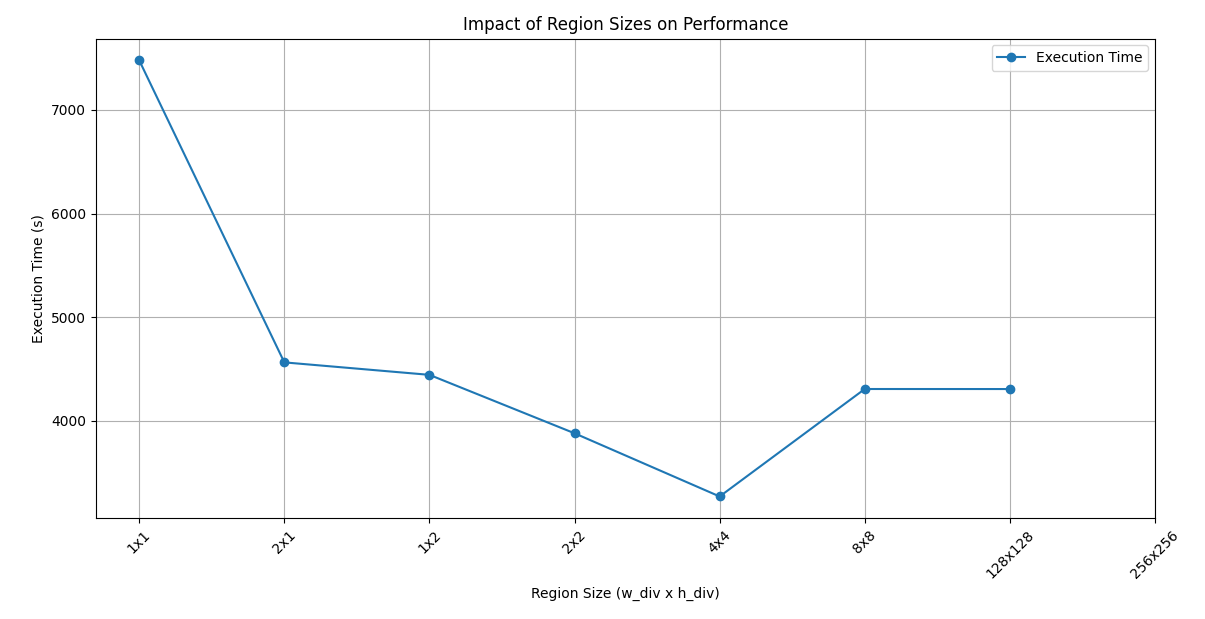
\includegraphics[width=0.8\textwidth]{./results/performance.png}
    \caption{Execution times for different parallelization strategies.}
    \label{fig:performance_plot}
\end{figure}

\begin{itemize}
    \item \textbf{(\(1 \times 1\)):}  
    No upscaling of performance was observed due to the lack of parallelism.
    
    \item \textbf{ (\(1 \times 2\) ; \(2 \times 1\)):}  
    Different performance results were observed between these configurations, likely due to variations in load balancing and the effect of splitting tasks into rows versus columns.
    
    \item \textbf{ (\(2 \times 2\) ; \(4 \times 4\)):}  
    These configurations showed a steady improvement in performance due to increased parallelization, with \(4 \times 4\) being the optimal setup for the virtual machine.
    
    \item \textbf{ (\(8 \times 8\)) ; \(128 \times 128\)):}  
    While small tiles offer higher parallelism by creating numerous independent tasks, the overhead of task management outweighs the benefits. This results in suboptimal performance.
    

    \item \textbf{ (\(256 \times 256\)):}  
    The \(256 \times 256\) tile size could not be executed due to limitations in the implementation: \textit{``The minimum region width and height is 4''}.
\end{itemize}

\noindent Based on the analysis, the \(4 \times 4\) tile size emerged as the optimal choice, offering 
a good balance of parallelism and efficiency for the virtual machine setup. 
The observed errors with larger tiles underscore the importance of carefully selecting region 
sizes compatible with the platform and application's requirements.
\vspace{-0.5em}


\end{document}